
\section{Overhead Analysis}
\label{sec::analysis}

In this section, we study the feasibility of the proposed IDRM protocol by estimating the
message overhead incurred by the protocol. 
%The exact overhead of IDRM depends on a variety of factors that are
%difficult to evaluate (e.g., MAC-layer management and oscillations due
%to conflicts of routing policies).  For clarity, we only consider the
%control overhead for maintaining network-layer information in
%intra-domain and inter-domain routing protocols.
Our analysis aims to convey a basic picture of the estimated overhead,
without involving the detailed steps of the protocol.
%For the clarity and convenience of analysis, 
We assume that no control packets are dropped or retransmitted, and
the inter-domain routing policies are simple, so that gateways will
not switch forwarding paths except when the paths are disconnected.
Our analysis follows a similar approach for analyzing proactive and reactive
routing protocols in \cite{CJV04overhead}.

%\vspace{-5pt} 
\begin{table}[htb!] \centering
        \begin{tabular}{|c||l|} \hline
        Symbol & Defintion \\
        \hline\hline
        ${N}$ & Total number of nodes in a domain \\
        ${G}$ & The number of gateways in a domain \\ 
        $r$  & Transmission radius \\ 
        $\bar{\nu}$ & Average speed of a node \\ 
        $\bar{E}$ & Average number of links in a domain \\ \hline	
        \end{tabular}  \label{tab:manet_def} 
        %\vspace{-8pt} 
\end{table} 


First, consider a single domain with the parameters as defined in
Table~\ref{tab:manet_def}.  Assume that the mobility process of nodes
is stationary and be confined to a bounded area. For a pair of nodes,
if one node moves out of the transmission radius of other, then the
link between them breaks. So, the average lifespan of a
link is
$\Theta\big(r\slash\bar{\nu}\big)$,
and the average number of link breakages per second due to mobility is
$\Theta\big(\bar{E}\bar{\nu}\slash r\big)$.

Since the mobility process of nodes is stationary where there is no net links
are created or broken over time, the average numbers of link creations
per second due to mobility in the domain is also
$\Theta\big(\bar{E}\bar{\nu}\slash r\big)$.  Hence, the
average number of link state changes (creations or breakages) per
second is $\Theta\big(\bar{E}\bar{\nu}\slash r\big)$.
The control overhead of intra-domain routing protocols is determined
by the number of link state changes. 

Next, we estimate the overhead for proactive intra-domain routing protocols, reactive intra-domain routing protocols, and inter-domain routing protocol, respectively.


(1) {\bf Proactive Intra-domain Routing Protocols:} Each node periodically broadcasts hello
packets to its neighbours. Based on the received hello packets, each node
announces a new link-state$\slash$distance-vector packet that will be
propagated throughout the MANET.
Let $\lambda^{\sf hel}$ be the number of hello packets broadcast by
each node per second. The total number of hello packets per second is
$\lambda^{\sf hel}   {N}$.

Since the average number of link state changes per second is
$\Theta\big(\bar{E}\bar{\nu}\slash r\big)$, the total
number of link-state$\slash$distance-vector packets per second broadcast  
is ${\rm O}\big(\bar{E}^2 \bar{\nu}\slash r\big)$.
This is an upper bound because optimized broadcast-based protocols
(e.g., OLSR) normally requires less than $\bar{E}$ transmissions
for each link-state$\slash$distance-vector packet to propagate
throughout the network.  Thus, the estimated number of control packets
per second is: %\vspace{-5pt}
\begin{equation} \label{eq:pro-oh}
\lambda^{\sf hel}   {N} + {\rm O}\big(\bar{E}^2 \bar{\nu}\slash r\big) %\vspace{-5pt}
\end{equation}
This is also the control overhead per second (at domain level) by IDRM 
to detect network partition and merging.



(2) {\bf Reactive Intra-domain Routing Protocols:} 
IDRM requires beaconing among gateways
to detect network partition or merging. The number of gateway pairs
that will beacon each other is upper bounded by
${\rm O}({G}^2)$.
Let $\lambda^{\sf bea}$ be the beaconing rate between a pair of
gateways. Then total number of beacons per second by
gateways is ${\rm O}(\lambda^{\sf bea} {G}^2)$.

Let $\bar{L}$ be the average number of hops between a pair of nodes in the MANET. The number of link state changes per second for a path between a pair of gateways is: 
$\Theta \big(\bar{L} \bar{\nu}\slash r\big)$.
Since each link state change will incur maintenance overhead in
reactive routing protocols, it is reasonable to assume that the number
of control packets is proportional to the number of link state changes and
the beaconing traffic.  Hence, the estimated number of control packets
per second required by IDRM to detect network partition and merging is: %\vspace{-5pt}
\begin{equation} \label{eq:rea-oh} 
{\rm O}\Big(\lambda^{\sf bea} {G}^2 \bar{L} \bar{\nu}\slash r\Big) %\vspace{-5pt}
\end{equation}



(3) {\bf Inter-domain Routing Protocol:}
Suppose there are $m^{\sf pro}$ domains running proactive routing
protocols and $m^{\sf rea}$ domains running reactive routing
protocols. Also assume each domain has the same parameters as in
Table~\ref{tab:manet_def}.
Note that the path vector protocol in IDRM behaves like a proactive routing
protocols, but with different parameters. Let $\lambda^{\sf inter}$
be the number of inter-domain hello packets broadcast by each gateway
per second in the path vector protocol. The total number of hello
packets generated in the multi-domain MANET per second is
$(m^{\sf pro} + m^{\sf rea})  \lambda^{\sf inter}  {\bar{G}}$,
where $\bar{G}$ denotes the average number of gateways in each domain.

If a pair of intra-domain gateways stay in the same MANET, there may be multiple
paths connecting them.  Let $1\slash\mu$ be the average lifespan of
the connectivity between a pair of intra-domain gateways. That is,
${\mu}$ is the connectivity breakage rate of connected pairs of intra-domain
gateways due to mobility. By stationarity of mobility process, ${\mu}$
is also the rate of change for the connectivity status of intra-domain
gateways.  Since IDRM will carry out new membership management and
announcement when the connectivity status between a pair of
intra-domain gateways is changed, the estimated number of connectivity
status changes is: %\vspace{-5pt}
\[ 
{\rm O}\Big((m^{\sf pro} + m^{\sf rea}) {\mu}  {\bar{G}}^2 \Big) %\vspace{-5pt}
\]
Hence, the total number of control packets per second for path vector protocol is: %\vspace{-5pt}
\begin{equation} \label{eq:pv-oh} 
 (m^{\sf pro} + m^{\sf rea}) \lambda^{\sf inter}   {\bar{G}} + {\rm O}\Big( (m^{\sf pro} + m^{\sf rea}) {\mu}   {\bar{G}}^2   \bar{E}^{\sf inter} \Big) %\vspace{-5pt}
\end{equation}
where $\bar{E}^{\sf inter}$ is the average number of pairs 
of connected inter-domain gateways in the $(m^{\sf pro} + m^{\sf rea})$ domains. 
%Clearly, $\bar{E}^{\sf inter} = {\rm O}(G^2)$.
%\[
%{\rm O}\Big((m^{\sf pro} + m^{\sf rea})   (\mu   {\bar{G}}^2 + \lambda^{\sf inter}   \bar{E}^{\sf inter})\Big)
%\]

In a given network, $m^{\sf pro}, m^{\sf rea}, \bar{G}, \bar{E}$, and
$\lambda^{\sf inter}$ are fixed. It is not straightforward to
decide $\mu$. But we can obtain this value from 
simulation. In Figure \ref{fig:mu_02},
%we plot the values of these
%two parameters that we have obtained for the network scenarios from
%our earlier discussion. We observe that
%$\bar{E}^{\sf inter} = {\rm O}(G^2)$. 
%Interestingly, however, 
we observe $\mu$ decreases as the
number of nodes increases because as a MANET becomes denser, the
connectivity between a pair of gateways becomes more stable, whereas
node speed adversely affects the stability of links almost linearly.  

\begin{figure}[htb!] \centering
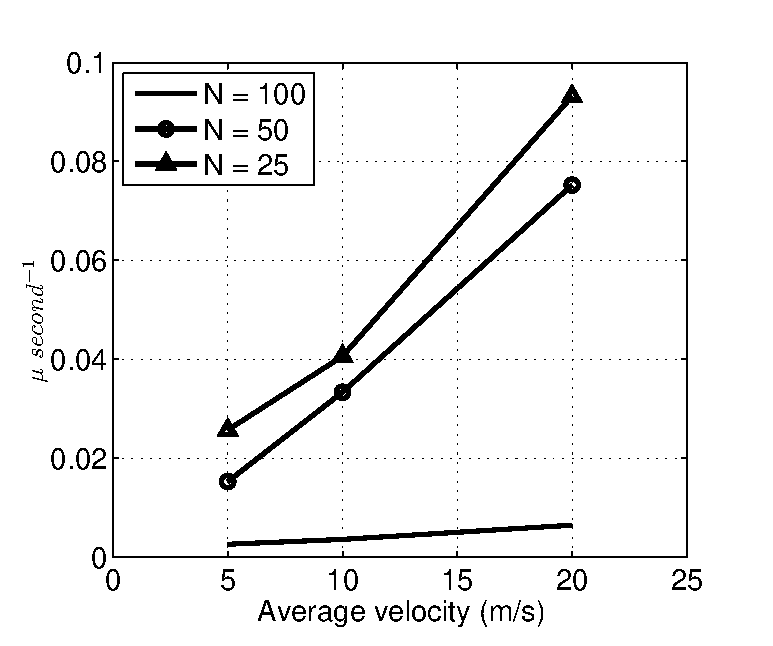
\includegraphics[width=0.35\textwidth, height=1.4in]{mu_vs_v_2} %\vspace{-10pt}
\caption{{\footnotesize Average lifespan of the connectivity between a pair of intra-domain gateways.}}
\label{fig:mu_02} %\vspace{-5pt}
\end{figure}


Note that Eq.~(\ref{eq:pv-oh}) only provides an asymptotic result for the
{\em total} control overhead incurred by IDRM without any
optimization. Since the overhead will be distributed among all the
gateways and various optimization can be applied (e.g., suppression of
hello, adaptive adjustment of probing interval), the overhead
incurred at each gateway for inter-domain routing operation will be
quite moderate.

We compare this estimation to the normal routing overhead
(not incurred by inter-domain routing). The overhead for proactive domains is Eq.~(\ref{eq:pro-oh}), and the same for reactive domains is Eq.~(\ref{eq:rea-oh}).
%Based on Equation X, for proactive domains, we have ({\bf Sid, please put Eq numbers})
%\[ 
%m^{\sf pro}   \lambda^{\sf hel}   {N} + {\rm O}\Big(m^{\sf pro}   \frac{\bar{\nu}}{r}  \bar{E}^2\Big).
%\]
%Based on Equation Y, for reactive domains, we have 
%\[
%{\rm O}\Big(m^{\sf rea}   \lambda^{\sf bea}   {G}^2   \frac{\bar{\nu}}{r}   \bar{L}\Big).
%\]
Note that $N$ and $\bar{E}$ are typically orders of magnitude greater
than the other parameters. Thus, the overhead from reactive domains
and inter-domain operations are substantially small compared to
proactive domains.


To summarize, in a multi-domain MANET consisting of proactive and reactive domains, the overall control overhead is dominated by that of the proactive domains, and the overhead incurred by inter-domain routing protocol is relatively insignificant. Thus we report that inter-domain routing can be supported with moderate additional overheads in MANETs, and IDRM is a viable approach to enable that.
%In conclusion, since the overhead incurred in proactive domains
%is intrinsic and independent of inter-domain routing, the extra overhead of IDRM will be
%relatively insignificant. %compared to the intrinsic overhead of proactive domains. 
%We conjecture it will be rather moderate even when many domains employ reactive routing but it depends on the actual configurations.


%% \subsubsection{Overall Overhead}

%% Therefore, the estimated total overhead of IDRM is composed of
%% intra-domain control packets and path vector protocol control packets,
%% namely,
%% \[
%% \begin{array}{r@{}l}
%% & m^{\sf pro}   \lambda^{\sf hel}   {N} + {\rm O}\Big(m^{\sf pro}   \frac{\bar{\nu}}{r}  \bar{E}^2\Big) + 
%% {\rm O}\Big(m^{\sf rea}   \lambda^{\sf bea}   {G}^2   \frac{\bar{\nu}}{r}   \bar{L}\Big) \\
%% + & \lambda^{\sf inter}   (m^{\sf pro} + m^{\sf rea})   {N} + {\rm O}\Big({\mu}   (m^{\sf pro} + m^{\sf rea})   {G}^2   \bar{E}^{\sf inter}\Big)
%% \end{array}
%% \]

%% Note that $\bar{E}, \bar{L}, \bar{n}$ depend on $N, r$, and $\bar{E}^{\sf inter}$ depends on $N, r, m^{\sf pro}, m^{\sf rea}, G$, whereas $\mu$ depends on $N, r, \bar{\nu}$. It is possible to control the overhead of IDRM by adjusting $N, r,$ $m^{\sf pro}, m^{\sf rea},$ $G, \bar{\nu}$. See Figures~\ref{fig:E_int} and \ref{fig:mu_02} for the empirical scaling behaviour of $\bar{E}^{\sf inter}$ and $\mu$, which are observed to only increase moderately (polynomial growth) as the gateways density and average speed of nodes. 

%% In general, based on our analysis we deduce that the overall overhead of IDRM only increases moderately as the gateways density and average speed of nodes, supporting the feasibility of IDRM.


%\begin{figure}[htb!] %\vspace{-10pt} \centering
%\includegraphics[width=0.4\textwidth, height=1.6in]{E_int} %\vspace{-10pt}
%\caption{{\footnotesize Average number of links between inter-domain gateways.}}
%\label{fig:E_int} %\vspace{-10pt}
%\end{figure}
